% Preamble

\documentclass{amsart}

%\usepackage{amssymb, amscd, amsfonts}
%\usepackage[mathscr]{eucal}
%\usepackage{graphicx}
\usepackage{lscape}
\usepackage{tikz}
\usepackage{scalefnt}
%\usepackage[applemac]{inputenc}
\usepackage[latin1]{inputenc}
%\usepackage[utf8x]{inputenc}
%\usepackage{verbatim}
%\usepackage[export]{adjustbox}
%\usepackage{lipsum}
\usepackage{float}% If comment this, figure moves to Page 2
\usepackage[pgf,outputdir={docgraphs/}]{dot2texi}
%\usepackage[active,tightpage]{preview}
\usetikzlibrary{shapes,automata,arrows}

\begin{document}

\title{Ricorrenze Locali}

\section{Ricorrenze Locali}

{\bigskip \bigskip \bigskip 
\subsection{Ricorrenza locale Grafo $P_1^{( 1)}\times P_8^{( 1)}$ } \

$$\scalefont{0.3}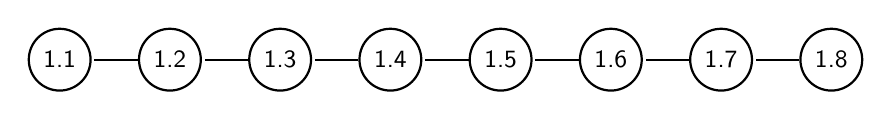
\begin{tikzpicture}
		 [,>=stealth',shorten >=1pt,auto,node distance=1.4cm,thick,main node/.style={circle,draw,font=\sffamily\small}] 
	\node[main node] (1) {1.1}; 
	\node[main node] (2) [right of=1] {1.2}; 
	\node[main node] (3) [right of=2] {1.3}; 
	\node[main node] (4) [right of=3] {1.4}; 
	\node[main node] (5) [right of=4] {1.5}; 
	\node[main node] (6) [right of=5] {1.6}; 
	\node[main node] (7) [right of=6] {1.7}; 
	\node[main node] (8) [right of=7] {1.8}; 

\path[every node/.style={font=\sffamily\small}] 
	(2) edge  node[above] {} (1) 
	(3) edge  node[above] {} (2) 
	(4) edge  node[above] {} (3) 
	(5) edge  node[above] {} (4) 
	(6) edge  node[above] {} (5) 
	(7) edge  node[above] {} (6) 
	(8) edge  node[above] {} (7) 
; 
\end{tikzpicture}$$

 $$\begin{tabular}{c | r r r r r r r}
$T(n,k)$&$k=0$&1&2&3&4&5&6\\ \hline 
$0$&1\\ 
$1$&1&1\\ 
$2$&1&2\\ 
$3$&1&3&1\\ 
$4$&1&4&3\\ 
$5$&1&5&6&1\\ 
$6$&1&6&10&4\\ 
$7$&1&7&15&10&1\\ 
$8$&1&8&21&20&5\\ 
$9$&1&9&28&35&15&1\\ 
$10$&1&10&36&56&35&6\\ 
$11$&1&11&45&84&70&21&1\\ 
\end{tabular}$$



\bigskip In questo caso otteniamo la \emph{ricorrenza locale} dal denominatore della funzione generatrice della somma delle righe:\par


$$F(x)=\frac{(-2 - x)}{(-1 + x + x^2)}\ .$$

$$\mbox{schema}\ \ \ 
\begin{tabular}{| c | c |} \hline 
${1}$&${0}$\\ \hline 
${0}$&${1}$\\ \hline 
${0}$&${*}$\\ \hline 
\end{tabular} $$\\

$$T(n,k)=T(n-1,k) + T(n-2,k-1)$$\newpage\subsection{Ricorrenza locale Grafo $P_1^{( 1)}\times P_8^{( 2)}$ } \

$$\scalefont{0.3}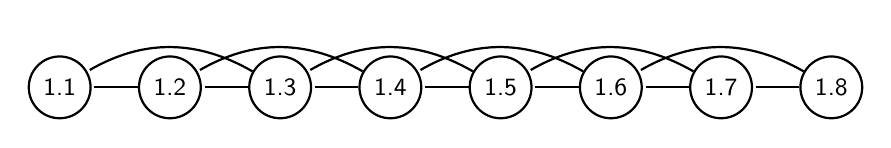
\begin{tikzpicture}
		 [,>=stealth',shorten >=1pt,auto,node distance=1.4cm,thick,main node/.style={circle,draw,font=\sffamily\small}] 
	\node[main node] (1) {1.1}; 
	\node[main node] (2) [right of=1] {1.2}; 
	\node[main node] (3) [right of=2] {1.3}; 
	\node[main node] (4) [right of=3] {1.4}; 
	\node[main node] (5) [right of=4] {1.5}; 
	\node[main node] (6) [right of=5] {1.6}; 
	\node[main node] (7) [right of=6] {1.7}; 
	\node[main node] (8) [right of=7] {1.8}; 

\path[every node/.style={font=\sffamily\small}] 
	(2) edge  node[above] {} (1) 
	(3) edge  node[above] {} (2) 
	(4) edge  node[above] {} (3) 
	(5) edge  node[above] {} (4) 
	(6) edge  node[above] {} (5) 
	(7) edge  node[above] {} (6) 
	(8) edge  node[above] {} (7) 
	(3) edge [bend right] node[above] {} (1) 
	(4) edge [bend right] node[above] {} (2) 
	(5) edge [bend right] node[above] {} (3) 
	(6) edge [bend right] node[above] {} (4) 
	(7) edge [bend right] node[above] {} (5) 
	(8) edge [bend right] node[above] {} (6) 
; 
\end{tikzpicture}$$

 $$\begin{tabular}{c | r r r r r}
$T(n,k)$&$k=0$&1&2&3&4\\ \hline 
$0$&1\\ 
$1$&1&1\\ 
$2$&1&2\\ 
$3$&1&3\\ 
$4$&1&4&1\\ 
$5$&1&5&3\\ 
$6$&1&6&6\\ 
$7$&1&7&10&1\\ 
$8$&1&8&15&4\\ 
$9$&1&9&21&10\\ 
$10$&1&10&28&20&1\\ 
$11$&1&11&36&35&5\\ 
\end{tabular}$$



\bigskip In questo caso otteniamo la \emph{ricorrenza locale} dal denominatore della funzione generatrice della somma delle righe:\par


$$F(x)=\frac{(-3 - x - 2x^2)}{(-1 + x + x^3)}\ .$$

$$\mbox{schema}\ \ \ 
\begin{tabular}{| c | c |} \hline 
${1}$&${0}$\\ \hline 
${0}$&${0}$\\ \hline 
${0}$&${1}$\\ \hline 
${0}$&${*}$\\ \hline 
\end{tabular} $$\\

$$T(n,k)=T(n-1,k) + T(n-3,k-1)$$\newpage\subsection{Ricorrenza locale Grafo $P_1^{( 1)}\times P_8^{( 3)}$ } \

$$\scalefont{0.3}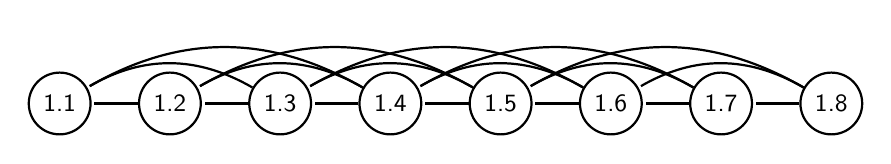
\begin{tikzpicture}
		 [,>=stealth',shorten >=1pt,auto,node distance=1.4cm,thick,main node/.style={circle,draw,font=\sffamily\small}] 
	\node[main node] (1) {1.1}; 
	\node[main node] (2) [right of=1] {1.2}; 
	\node[main node] (3) [right of=2] {1.3}; 
	\node[main node] (4) [right of=3] {1.4}; 
	\node[main node] (5) [right of=4] {1.5}; 
	\node[main node] (6) [right of=5] {1.6}; 
	\node[main node] (7) [right of=6] {1.7}; 
	\node[main node] (8) [right of=7] {1.8}; 

\path[every node/.style={font=\sffamily\small}] 
	(2) edge  node[above] {} (1) 
	(3) edge  node[above] {} (2) 
	(4) edge  node[above] {} (3) 
	(5) edge  node[above] {} (4) 
	(6) edge  node[above] {} (5) 
	(7) edge  node[above] {} (6) 
	(8) edge  node[above] {} (7) 
	(3) edge [bend right] node[above] {} (1) 
	(4) edge [bend right] node[above] {} (2) 
	(5) edge [bend right] node[above] {} (3) 
	(6) edge [bend right] node[above] {} (4) 
	(7) edge [bend right] node[above] {} (5) 
	(8) edge [bend right] node[above] {} (6) 
	(4) edge [bend right] node[above] {} (1) 
	(5) edge [bend right] node[above] {} (2) 
	(6) edge [bend right] node[above] {} (3) 
	(7) edge [bend right] node[above] {} (4) 
	(8) edge [bend right] node[above] {} (5) 
; 
\end{tikzpicture}$$

 $$\begin{tabular}{c | r r r r}
$T(n,k)$&$k=0$&1&2&3\\ \hline 
$0$&1\\ 
$1$&1&1\\ 
$2$&1&2\\ 
$3$&1&3\\ 
$4$&1&4\\ 
$5$&1&5&1\\ 
$6$&1&6&3\\ 
$7$&1&7&6\\ 
$8$&1&8&10\\ 
$9$&1&9&15&1\\ 
$10$&1&10&21&4\\ 
$11$&1&11&28&10\\ 
\end{tabular}$$



\bigskip In questo caso otteniamo la \emph{ricorrenza locale} dal denominatore della funzione generatrice della somma delle righe:\par


$$F(x)=\frac{(-4 - x - 2x^2 - 3x^3)}{(-1 + x + x^4)}\ .$$

$$\mbox{schema}\ \ \ 
\begin{tabular}{| c | c |} \hline 
${1}$&${0}$\\ \hline 
${0}$&${0}$\\ \hline 
${0}$&${0}$\\ \hline 
${0}$&${1}$\\ \hline 
${0}$&${*}$\\ \hline 
\end{tabular} $$\\

$$T(n,k)=T(n-1,k) + T(n-4,k-1)$$\newpage\subsection{Ricorrenza locale Grafo $P_1^{( 1)}\times P_8^{(e 3)}$ } \

$$\scalefont{0.3}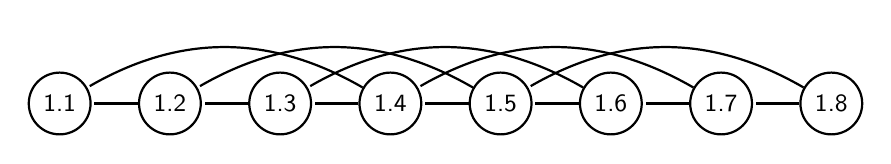
\begin{tikzpicture}
		 [,>=stealth',shorten >=1pt,auto,node distance=1.4cm,thick,main node/.style={circle,draw,font=\sffamily\small}] 
	\node[main node] (1) {1.1}; 
	\node[main node] (2) [right of=1] {1.2}; 
	\node[main node] (3) [right of=2] {1.3}; 
	\node[main node] (4) [right of=3] {1.4}; 
	\node[main node] (5) [right of=4] {1.5}; 
	\node[main node] (6) [right of=5] {1.6}; 
	\node[main node] (7) [right of=6] {1.7}; 
	\node[main node] (8) [right of=7] {1.8}; 

\path[every node/.style={font=\sffamily\small}] 
	(2) edge  node[above] {} (1) 
	(3) edge  node[above] {} (2) 
	(4) edge  node[above] {} (3) 
	(5) edge  node[above] {} (4) 
	(6) edge  node[above] {} (5) 
	(7) edge  node[above] {} (6) 
	(8) edge  node[above] {} (7) 
	(4) edge [bend right] node[above] {} (1) 
	(5) edge [bend right] node[above] {} (2) 
	(6) edge [bend right] node[above] {} (3) 
	(7) edge [bend right] node[above] {} (4) 
	(8) edge [bend right] node[above] {} (5) 
; 
\end{tikzpicture}$$

 $$\begin{tabular}{c | r r r r r r r}
$T(n,k)$&$k=0$&1&2&3&4&5&6\\ \hline 
$0$&1\\ 
$1$&1&1\\ 
$2$&1&2\\ 
$3$&1&3&1\\ 
$4$&1&4&2\\ 
$5$&1&5&4&1\\ 
$6$&1&6&7&2\\ 
$7$&1&7&11&5&1\\ 
$8$&1&8&16&10&2\\ 
$9$&1&9&22&18&6&1\\ 
$10$&1&10&29&30&13&2\\ 
$11$&1&11&37&47&26&7&1\\ 
\end{tabular}$$



\bigskip In questo caso otteniamo la \emph{ricorrenza locale} dal denominatore della funzione generatrice della somma delle righe:\par


$$F(x)=\frac{(-5 - 2x + x^2 - 3x^3)}{(-1 + x + x^2 - x^3 + x^4)}\ .$$

$$\mbox{schema}\ \ \ 
\begin{tabular}{| c | c |} \hline 
${1}$&${0}$\\ \hline 
${-1}$&${0}$\\ \hline 
${1}$&${0}$\\ \hline 
${0}$&${1}$\\ \hline 
${0}$&${*}$\\ \hline 
\end{tabular} $$\\

$$T(n,k)=T(n-1,k) + T(n-2,k-1) - T(n-3,k-1) + T(n-4,k-1)$$\newpage\subsection{Ricorrenza locale Grafo $P_2^{( 1)}\times P_7^{( 1)}$ } \

$$\scalefont{0.3}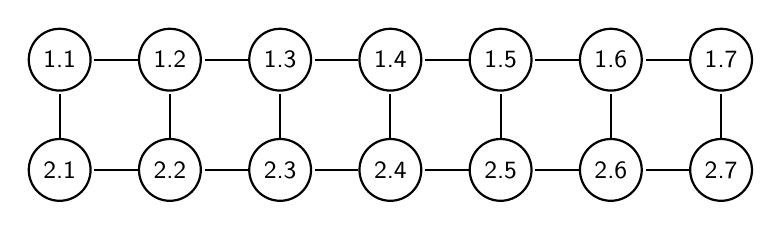
\begin{tikzpicture}
		 [,>=stealth',shorten >=1pt,auto,node distance=1.4cm,thick,main node/.style={circle,draw,font=\sffamily\small}] 
	\node[main node] (1) {1.1}; 
	\node[main node] (2) [below of=1] {2.1}; 
	\node[main node] (3) [right of=1] {1.2}; 
	\node[main node] (4) [right of=2] {2.2}; 
	\node[main node] (5) [right of=3] {1.3}; 
	\node[main node] (6) [right of=4] {2.3}; 
	\node[main node] (7) [right of=5] {1.4}; 
	\node[main node] (8) [right of=6] {2.4}; 
	\node[main node] (9) [right of=7] {1.5}; 
	\node[main node] (10) [right of=8] {2.5}; 
	\node[main node] (11) [right of=9] {1.6}; 
	\node[main node] (12) [right of=10] {2.6}; 
	\node[main node] (13) [right of=11] {1.7}; 
	\node[main node] (14) [right of=12] {2.7}; 

\path[every node/.style={font=\sffamily\small}] 
	(2) edge  node[above] {} (1) 
	(4) edge  node[above] {} (3) 
	(6) edge  node[above] {} (5) 
	(8) edge  node[above] {} (7) 
	(10) edge  node[above] {} (9) 
	(12) edge  node[above] {} (11) 
	(14) edge  node[above] {} (13) 
	(3) edge  node[above] {} (1) 
	(5) edge  node[above] {} (3) 
	(7) edge  node[above] {} (5) 
	(9) edge  node[above] {} (7) 
	(11) edge  node[above] {} (9) 
	(13) edge  node[above] {} (11) 
	(4) edge  node[above] {} (2) 
	(6) edge  node[above] {} (4) 
	(8) edge  node[above] {} (6) 
	(10) edge  node[above] {} (8) 
	(12) edge  node[above] {} (10) 
	(14) edge  node[above] {} (12) 
; 
\end{tikzpicture}$$

 $$\begin{tabular}{c | r r r r r r r r}
$T(n,k)$&$k=0$&1&2&3&4&5&6&7\\ \hline 
$0$&1\\ 
$1$&1&2\\ 
$2$&1&4&2\\ 
$3$&1&6&8&2\\ 
$4$&1&8&18&12&2\\ 
$5$&1&10&32&38&16&2\\ 
$6$&1&12&50&88&66&20&2\\ 
$7$&1&14&72&170&192&102&24&2\\ 
\end{tabular}$$



\bigskip In questo caso otteniamo la \emph{ricorrenza locale} dal denominatore della funzione generatrice della somma delle righe:\par


$$F(x)=\frac{(-3 - x)}{(-1 + 2x + x^2)}\ .$$

$$\mbox{schema}\ \ \ 
\begin{tabular}{| c | c |} \hline 
${1}$&${0}$\\ \hline 
${1}$&${1}$\\ \hline 
${0}$&${*}$\\ \hline 
\end{tabular} $$\\

$$T(n,k)=T(n-1,k) + T(n-1,k-1) + T(n-2,k-1)$$\newpage\subsection{Ricorrenza locale Grafo $P_2^{( 1)}\times P_7^{( 2)}$ } \

$$\scalefont{0.3}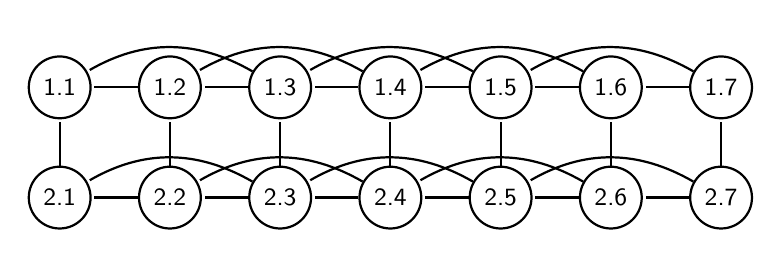
\begin{tikzpicture}
		 [,>=stealth',shorten >=1pt,auto,node distance=1.4cm,thick,main node/.style={circle,draw,font=\sffamily\small}] 
	\node[main node] (1) {1.1}; 
	\node[main node] (2) [below of=1] {2.1}; 
	\node[main node] (3) [right of=1] {1.2}; 
	\node[main node] (4) [right of=2] {2.2}; 
	\node[main node] (5) [right of=3] {1.3}; 
	\node[main node] (6) [right of=4] {2.3}; 
	\node[main node] (7) [right of=5] {1.4}; 
	\node[main node] (8) [right of=6] {2.4}; 
	\node[main node] (9) [right of=7] {1.5}; 
	\node[main node] (10) [right of=8] {2.5}; 
	\node[main node] (11) [right of=9] {1.6}; 
	\node[main node] (12) [right of=10] {2.6}; 
	\node[main node] (13) [right of=11] {1.7}; 
	\node[main node] (14) [right of=12] {2.7}; 

\path[every node/.style={font=\sffamily\small}] 
	(2) edge  node[above] {} (1) 
	(4) edge  node[above] {} (3) 
	(6) edge  node[above] {} (5) 
	(8) edge  node[above] {} (7) 
	(10) edge  node[above] {} (9) 
	(12) edge  node[above] {} (11) 
	(14) edge  node[above] {} (13) 
	(3) edge  node[above] {} (1) 
	(5) edge  node[above] {} (3) 
	(7) edge  node[above] {} (5) 
	(9) edge  node[above] {} (7) 
	(11) edge  node[above] {} (9) 
	(13) edge  node[above] {} (11) 
	(4) edge  node[above] {} (2) 
	(6) edge  node[above] {} (4) 
	(8) edge  node[above] {} (6) 
	(10) edge  node[above] {} (8) 
	(12) edge  node[above] {} (10) 
	(14) edge  node[above] {} (12) 
	(5) edge [bend right] node[above] {} (1) 
	(7) edge [bend right] node[above] {} (3) 
	(9) edge [bend right] node[above] {} (5) 
	(11) edge [bend right] node[above] {} (7) 
	(13) edge [bend right] node[above] {} (9) 
	(6) edge [bend right] node[above] {} (2) 
	(8) edge [bend right] node[above] {} (4) 
	(10) edge [bend right] node[above] {} (6) 
	(12) edge [bend right] node[above] {} (8) 
	(14) edge [bend right] node[above] {} (10) 
; 
\end{tikzpicture}$$

 $$\begin{tabular}{c | r r r r r r}
$T(n,k)$&$k=0$&1&2&3&4&5\\ \hline 
$0$&1\\ 
$1$&1&2\\ 
$2$&1&4&2\\ 
$3$&1&6&6\\ 
$4$&1&8&14&4\\ 
$5$&1&10&26&18&2\\ 
$6$&1&12&42&48&14\\ 
$7$&1&14&62&102&56&6\\ 
\end{tabular}$$



\bigskip In questo caso otteniamo la \emph{ricorrenza locale} dal denominatore della funzione generatrice della somma delle righe:\par


$$F(x)=\frac{(-7 - 6x - 7x^2 - 3x^3)}{(-1 + x + x^2 + 2x^3 + x^4)}\ .$$

$$\mbox{schema}\ \ \ 
\begin{tabular}{| c | c | c |} \hline 
${1}$&${0}$&${0}$\\ \hline 
${1}$&${1}$&${0}$\\ \hline 
${0}$&${1}$&${0}$\\ \hline 
${0}$&${0}$&${1}$\\ \hline 
${0}$&${0}$&${*}$\\ \hline 
\end{tabular} $$\\

$$T(n,k)=T(n-1,k) + T(n-2,k-1) + T(n-3,k-1) + T(n-3,k-2) + T(n-4,k-2)$$\newpage\subsection{Ricorrenza locale Grafo $P_2^{( 1)}\times Z_7^{( 1)}$ } \

$$\scalefont{0.3}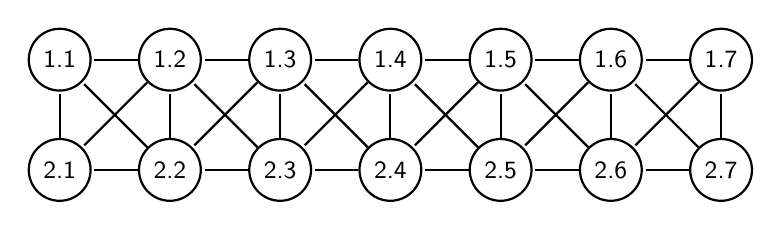
\begin{tikzpicture}
		 [,>=stealth',shorten >=1pt,auto,node distance=1.4cm,thick,main node/.style={circle,draw,font=\sffamily\small}] 
	\node[main node] (1) {1.1}; 
	\node[main node] (2) [below of=1] {2.1}; 
	\node[main node] (3) [right of=1] {1.2}; 
	\node[main node] (4) [right of=2] {2.2}; 
	\node[main node] (5) [right of=3] {1.3}; 
	\node[main node] (6) [right of=4] {2.3}; 
	\node[main node] (7) [right of=5] {1.4}; 
	\node[main node] (8) [right of=6] {2.4}; 
	\node[main node] (9) [right of=7] {1.5}; 
	\node[main node] (10) [right of=8] {2.5}; 
	\node[main node] (11) [right of=9] {1.6}; 
	\node[main node] (12) [right of=10] {2.6}; 
	\node[main node] (13) [right of=11] {1.7}; 
	\node[main node] (14) [right of=12] {2.7}; 
 \path[every node/.style={font=\sffamily\small}] 	(2) edge  node[above] {} (1) 
	(4) edge  node[above] {} (3) 
	(6) edge  node[above] {} (5) 
	(8) edge  node[above] {} (7) 
	(10) edge  node[above] {} (9) 
	(12) edge  node[above] {} (11) 
	(14) edge  node[above] {} (13) 
	(3) edge  node[above] {} (1) 
	(5) edge  node[above] {} (3) 
	(7) edge  node[above] {} (5) 
	(9) edge  node[above] {} (7) 
	(11) edge  node[above] {} (9) 
	(13) edge  node[above] {} (11) 
	(4) edge  node[above] {} (2) 
	(6) edge  node[above] {} (4) 
	(8) edge  node[above] {} (6) 
	(10) edge  node[above] {} (8) 
	(12) edge  node[above] {} (10) 
	(14) edge  node[above] {} (12) 
(3) edge [] node[above] {} (2)(4) edge [] node[above] {} (1)(5) edge [] node[above] {} (4)(6) edge [] node[above] {} (3)(7) edge [] node[above] {} (6)(8) edge [] node[above] {} (5)(9) edge [] node[above] {} (8)(10) edge [] node[above] {} (7)(11) edge [] node[above] {} (10)(12) edge [] node[above] {} (9)(13) edge [] node[above] {} (12)(14) edge [] node[above] {} (11); \end{tikzpicture}$$ $$\begin{tabular}{c | r r r r r}
$T(n,k)$&$k=0$&1&2&3&4\\ \hline 
$0$&1\\ 
$1$&1&2\\ 
$2$&1&4\\ 
$3$&1&6&4\\ 
$4$&1&8&12\\ 
$5$&1&10&24&8\\ 
$6$&1&12&40&32\\ 
$7$&1&14&60&80&16\\ 
\end{tabular}$$



\bigskip In questo caso otteniamo la \emph{ricorrenza locale} dal denominatore della funzione generatrice della somma delle righe:\par


$$F(x)=\frac{(-3 - 2x)}{(-1 + x + 2x^2)}\ .$$

$$\mbox{schema}\ \ \ 
\begin{tabular}{| c | c |} \hline 
${2}$&${0}$\\ \hline 
${0}$&${1}$\\ \hline 
${0}$&${*}$\\ \hline 
\end{tabular} $$\\

$$T(n,k)=T(n-1,k) + 2 T(n-2,k-1)$$\newpage\subsection{Ricorrenza locale Grafo $P_2^{( 1)}\times Z_7^{( 2)}$ } \

$$\scalefont{0.3}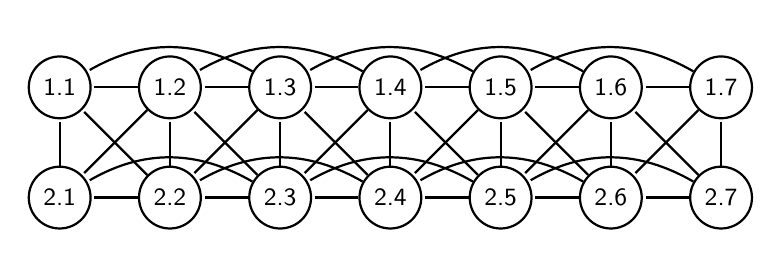
\begin{tikzpicture}
		 [,>=stealth',shorten >=1pt,auto,node distance=1.4cm,thick,main node/.style={circle,draw,font=\sffamily\small}] 
	\node[main node] (1) {1.1}; 
	\node[main node] (2) [below of=1] {2.1}; 
	\node[main node] (3) [right of=1] {1.2}; 
	\node[main node] (4) [right of=2] {2.2}; 
	\node[main node] (5) [right of=3] {1.3}; 
	\node[main node] (6) [right of=4] {2.3}; 
	\node[main node] (7) [right of=5] {1.4}; 
	\node[main node] (8) [right of=6] {2.4}; 
	\node[main node] (9) [right of=7] {1.5}; 
	\node[main node] (10) [right of=8] {2.5}; 
	\node[main node] (11) [right of=9] {1.6}; 
	\node[main node] (12) [right of=10] {2.6}; 
	\node[main node] (13) [right of=11] {1.7}; 
	\node[main node] (14) [right of=12] {2.7}; 
 \path[every node/.style={font=\sffamily\small}] 	(2) edge  node[above] {} (1) 
	(4) edge  node[above] {} (3) 
	(6) edge  node[above] {} (5) 
	(8) edge  node[above] {} (7) 
	(10) edge  node[above] {} (9) 
	(12) edge  node[above] {} (11) 
	(14) edge  node[above] {} (13) 
	(3) edge  node[above] {} (1) 
	(5) edge  node[above] {} (3) 
	(7) edge  node[above] {} (5) 
	(9) edge  node[above] {} (7) 
	(11) edge  node[above] {} (9) 
	(13) edge  node[above] {} (11) 
	(4) edge  node[above] {} (2) 
	(6) edge  node[above] {} (4) 
	(8) edge  node[above] {} (6) 
	(10) edge  node[above] {} (8) 
	(12) edge  node[above] {} (10) 
	(14) edge  node[above] {} (12) 
	(5) edge [bend right] node[above] {} (1) 
	(7) edge [bend right] node[above] {} (3) 
	(9) edge [bend right] node[above] {} (5) 
	(11) edge [bend right] node[above] {} (7) 
	(13) edge [bend right] node[above] {} (9) 
	(6) edge [bend right] node[above] {} (2) 
	(8) edge [bend right] node[above] {} (4) 
	(10) edge [bend right] node[above] {} (6) 
	(12) edge [bend right] node[above] {} (8) 
	(14) edge [bend right] node[above] {} (10) 
(3) edge [] node[above] {} (2)(4) edge [] node[above] {} (1)(5) edge [] node[above] {} (4)(6) edge [] node[above] {} (3)(7) edge [] node[above] {} (6)(8) edge [] node[above] {} (5)(9) edge [] node[above] {} (8)(10) edge [] node[above] {} (7)(11) edge [] node[above] {} (10)(12) edge [] node[above] {} (9)(13) edge [] node[above] {} (12)(14) edge [] node[above] {} (11); \end{tikzpicture}$$ $$\begin{tabular}{c | r r r r r}
$T(n,k)$&$k=0$&1&2&3&4\\ \hline 
$0$&1\\ 
$1$&1&2\\ 
$2$&1&4\\ 
$3$&1&6&2\\ 
$4$&1&8&8\\ 
$5$&1&10&18&2\\ 
$6$&1&12&32&12\\ 
$7$&1&14&50&38&2\\ 
\end{tabular}$$



\bigskip In questo caso otteniamo la \emph{ricorrenza locale} dal denominatore della funzione generatrice della somma delle righe:\par


$$F(x)=\frac{(-5 - 4x - 3x^2)}{(-1 + x + x^2 + x^3)}\ .$$

$$\mbox{schema}\ \ \ 
\begin{tabular}{| c | c |} \hline 
${1}$&${0}$\\ \hline 
${1}$&${0}$\\ \hline 
${0}$&${1}$\\ \hline 
${0}$&${*}$\\ \hline 
\end{tabular} $$\\

$$T(n,k)=T(n-1,k) + T(n-2,k-1) + T(n-3,k-1)$$\newpage\subsection{Ricorrenza locale Grafo $P_2^{( 1)}\times F_7^{( 1)}$ } \

$$\scalefont{0.3}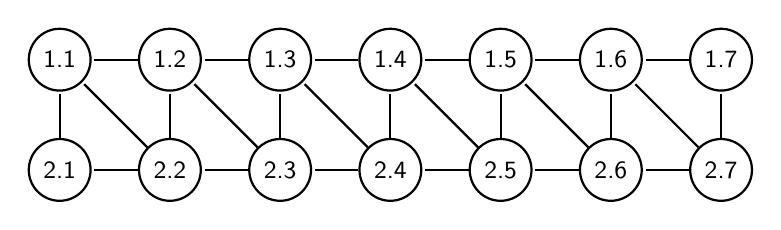
\begin{tikzpicture}
		 [,>=stealth',shorten >=1pt,auto,node distance=1.4cm,thick,main node/.style={circle,draw,font=\sffamily\small}] 
	\node[main node] (1) {1.1}; 
	\node[main node] (2) [below of=1] {2.1}; 
	\node[main node] (3) [right of=1] {1.2}; 
	\node[main node] (4) [right of=2] {2.2}; 
	\node[main node] (5) [right of=3] {1.3}; 
	\node[main node] (6) [right of=4] {2.3}; 
	\node[main node] (7) [right of=5] {1.4}; 
	\node[main node] (8) [right of=6] {2.4}; 
	\node[main node] (9) [right of=7] {1.5}; 
	\node[main node] (10) [right of=8] {2.5}; 
	\node[main node] (11) [right of=9] {1.6}; 
	\node[main node] (12) [right of=10] {2.6}; 
	\node[main node] (13) [right of=11] {1.7}; 
	\node[main node] (14) [right of=12] {2.7}; 
 \path[every node/.style={font=\sffamily\small}] 	(2) edge  node[above] {} (1) 
	(4) edge  node[above] {} (3) 
	(6) edge  node[above] {} (5) 
	(8) edge  node[above] {} (7) 
	(10) edge  node[above] {} (9) 
	(12) edge  node[above] {} (11) 
	(14) edge  node[above] {} (13) 
	(3) edge  node[above] {} (1) 
	(5) edge  node[above] {} (3) 
	(7) edge  node[above] {} (5) 
	(9) edge  node[above] {} (7) 
	(11) edge  node[above] {} (9) 
	(13) edge  node[above] {} (11) 
	(4) edge  node[above] {} (2) 
	(6) edge  node[above] {} (4) 
	(8) edge  node[above] {} (6) 
	(10) edge  node[above] {} (8) 
	(12) edge  node[above] {} (10) 
	(14) edge  node[above] {} (12) 
(4) edge [] node[above] {} (1)(6) edge [] node[above] {} (3)(8) edge [] node[above] {} (5)(10) edge [] node[above] {} (7)(12) edge [] node[above] {} (9)(14) edge [] node[above] {} (11); \end{tikzpicture}$$ $$\begin{tabular}{c | r r r r r r}
$T(n,k)$&$k=0$&1&2&3&4&5\\ \hline 
$0$&1\\ 
$1$&1&2\\ 
$2$&1&4&1\\ 
$3$&1&6&6\\ 
$4$&1&8&15&4\\ 
$5$&1&10&28&20&1\\ 
$6$&1&12&45&56&15\\ 
$7$&1&14&66&120&70&6\\ 
\end{tabular}$$



\bigskip In questo caso otteniamo la \emph{ricorrenza locale} dal denominatore della funzione generatrice della somma delle righe:\par


$$F(x)=\frac{(-3 - 3x - x^2)}{(-1 + x + 2x^2 + x^3)}\ .$$

$$\mbox{schema}\ \ \ 
\begin{tabular}{| c | c | c |} \hline 
${1}$&${0}$&${0}$\\ \hline 
${0}$&${2}$&${0}$\\ \hline 
${0}$&${0}$&${1}$\\ \hline 
${0}$&${0}$&${*}$\\ \hline 
\end{tabular} $$\\

$$T(n,k)=T(n-1,k) + 2 T(n-2,k-1) + T(n-3,k-2)$$\newpage} 

\end{document} 